% vim: spelllang=en spell textwidth=120
\documentclass[deska]{subfiles}
\begin{document}

\chapter{Server part of Deska}
\label{sec:deska-server}

\begin{abstract}
Talk about server part of Deska application. Deska server application and Deska database.
\end{abstract}

\section{Server and its database}
Server part of Deska application can be divided into two parts. The {\em Deska server} and {\em Deska database}.
Deska server is python application, that runs for every user, listens for the commands from deska-cli (see DBAPI protocol).
Main work is to load JSON data, call corresponding database function, and return the answer to deska-cli.
There are some special functions (freezeChangeset, showConfigDiff etc.) that are not implemented by Deska database, but the server itselfs.
The last part of Deska server work is to run Configuration generators.\\
Due to the fact that the user defined schemas are modular, the most of stored procedures which are called by server have to be generated to fit with the schema.
These functions and tables are genearated by SQL generator (see \secref{sec:sql-generator}) during installation of the Deska database. How the generated functions and tables work together to fulfil excpectations from DBAPI (see~\secref{sec:dbapi-protocol}) is described in \secref{sec:deska-db-data-manipulation}.

\section{Deska server}
\label{sec:server-py}

This section talks about deska-server, python application providing interaction with database.

\todo{Honza: when it is start, parameters}

\subsection{Database connection}
After Deska server start, it tries to connect to Deska database using Psycopg2 python modul.
Parameters of connection are taken from Deska server parameters on start.
When connection is successfull, it is kept until Deska server is terminated.

\subsection{Command running}
For communication with the {\tt deska-cli}, the JSON-based DBAPI (see~\secref{sec:dbapi-protocol} is used. On server side, this JSON is tranformed into python structure of dicts and lists. Some check are performed, like if command or number of arguments is right.
Most of command have their implementation inside the database, so the proper db function is called and its result is retuned. In this part, there is no special logic, just check parameter, add some defaults if it is needed and catch db exceptions.

But there are some function implemented in deska-server, like function for view freezing, which just starts or ends transaction, with isolation
level read committed, to perform the freezing of view.
Also showConfigDiff is not implemented in database. Special is commitChangeset, which has database implementation,
but also needs to do generation of configuration outside the database (similar to showConfigDiff).
These two functions that runs Configuration genarators (\secref{sec:config-generators}), works with read commited isolation level transakction.
At first commitChangeset in Deska database is run, than Configuration generator produced configuration.
At the end, in showConfigDiff is database transaction aborted. In commitChangeset only if error in
Configuration generators occurs. Therefore Configuration generators can access resolved data from
production tables in database, as decribed in \secref{sec:direct-access}

The combination of these 2 types is applyBatchedChangeset, which start transaction at begin, then perform its arguments, as it was a single
command, and then commit (or abort) the transaction. 
Function that calls only one database function, pass the result because it is already in proper JSON format, but if the function does some
more computing outside the database, or not call db function at all, it must create the result by its own.

\subsection{Security Model}
\label{sec:server-security-model}

The {\tt deska-server} relies heavily on the authentication/authorization features offered by the SSH server, and on the
{\tt trust = ident} feature of the PostgreSQL server.  Any Unix user who is able to connect to the PostgreSQL database
which contains the Deska installation will be able to perform any modification to the database over the standard DBAPI
calls.

\todo{Lukas: exceptions on server}

\section{Deska database}
Deska-database is Postgresql database server, storing all data of user given schema, its relations and all changes of data.
There are tables, specified by user before build Deska database, tables for history tracking and many function for data manipulation.

\subsection{Data storage}
To prevent misunderstanding, if we talk about database, we use word {\em schema} in two different meanings. {\em User defined schema},
with meaning tables, with constraints describing data, that user wants to store into database. And {\em schema}, term used by
Postgresql with meaning something as namespace containing database objects (tables, types, functions etc).
If we talk about user defined schema, we write the whole term, and if we talk about schema, we write
schema plus its name.

Lets look at how data are stored in Deska database. Three types of data are stored in Deska database.

\subsubsection{Deska database schema} 
Firstly there are information about user defined database schema. These information are provided by {\tt kindNames}, {\tt kindAttributes} and {\tt kindRelations} functions.
These information are read from database catalog and stored in {\tt generated.py} file. This file is used by functions listed above to get asked information. So later it is not needed to access the database catalog or any table.

\subsubsection{Objects stored in Deska database}
Secondly, the why we are here - the meaning of life, user data, fitting into user defined schema.
Objects and its attributes are stored in tables. 
After changeset is started, all data inserted into database, are placed into tables in history schema. Every kind has table in history
schema, with all attributes defined in user defined schema, and some more for history tracking.
Tables defined by user are created in schema production. These tables
(with its constraints) are used for data validation when committing changeset. If data are successfully copied into tables in schema production
from tables in schema history, data are valid against the user defined schema.
See \secref{sec:versioning} for more info.

\subsubsection{Revisions and changesets}
Thirdly, information about revisions and changeset. There are two tables, version (the name was here before
we start using {\em revision}) and changeset, for storing information about revisions and changesets. These tables are
in versioning schema.

\subsection{Data manipulation}
There are many stored procedures for manipulation with stored data, in Postgresql called {\em functions}.
Every action with data, as create object, set attribute, delete object, get object data, create changeset, delete changeset etc.,
has a function that do that. These functions for object and its attributes are generated by SQL generator (see \secref{sec:sql-generator}) in genproc schema.
The functions for getting information about changesets and versions are written by hand and stored in Deska schema with many auxiliary functions.

\subsection{Communication}
\begin{figure}[h]
	\centering
	\label{img:deska-server}
	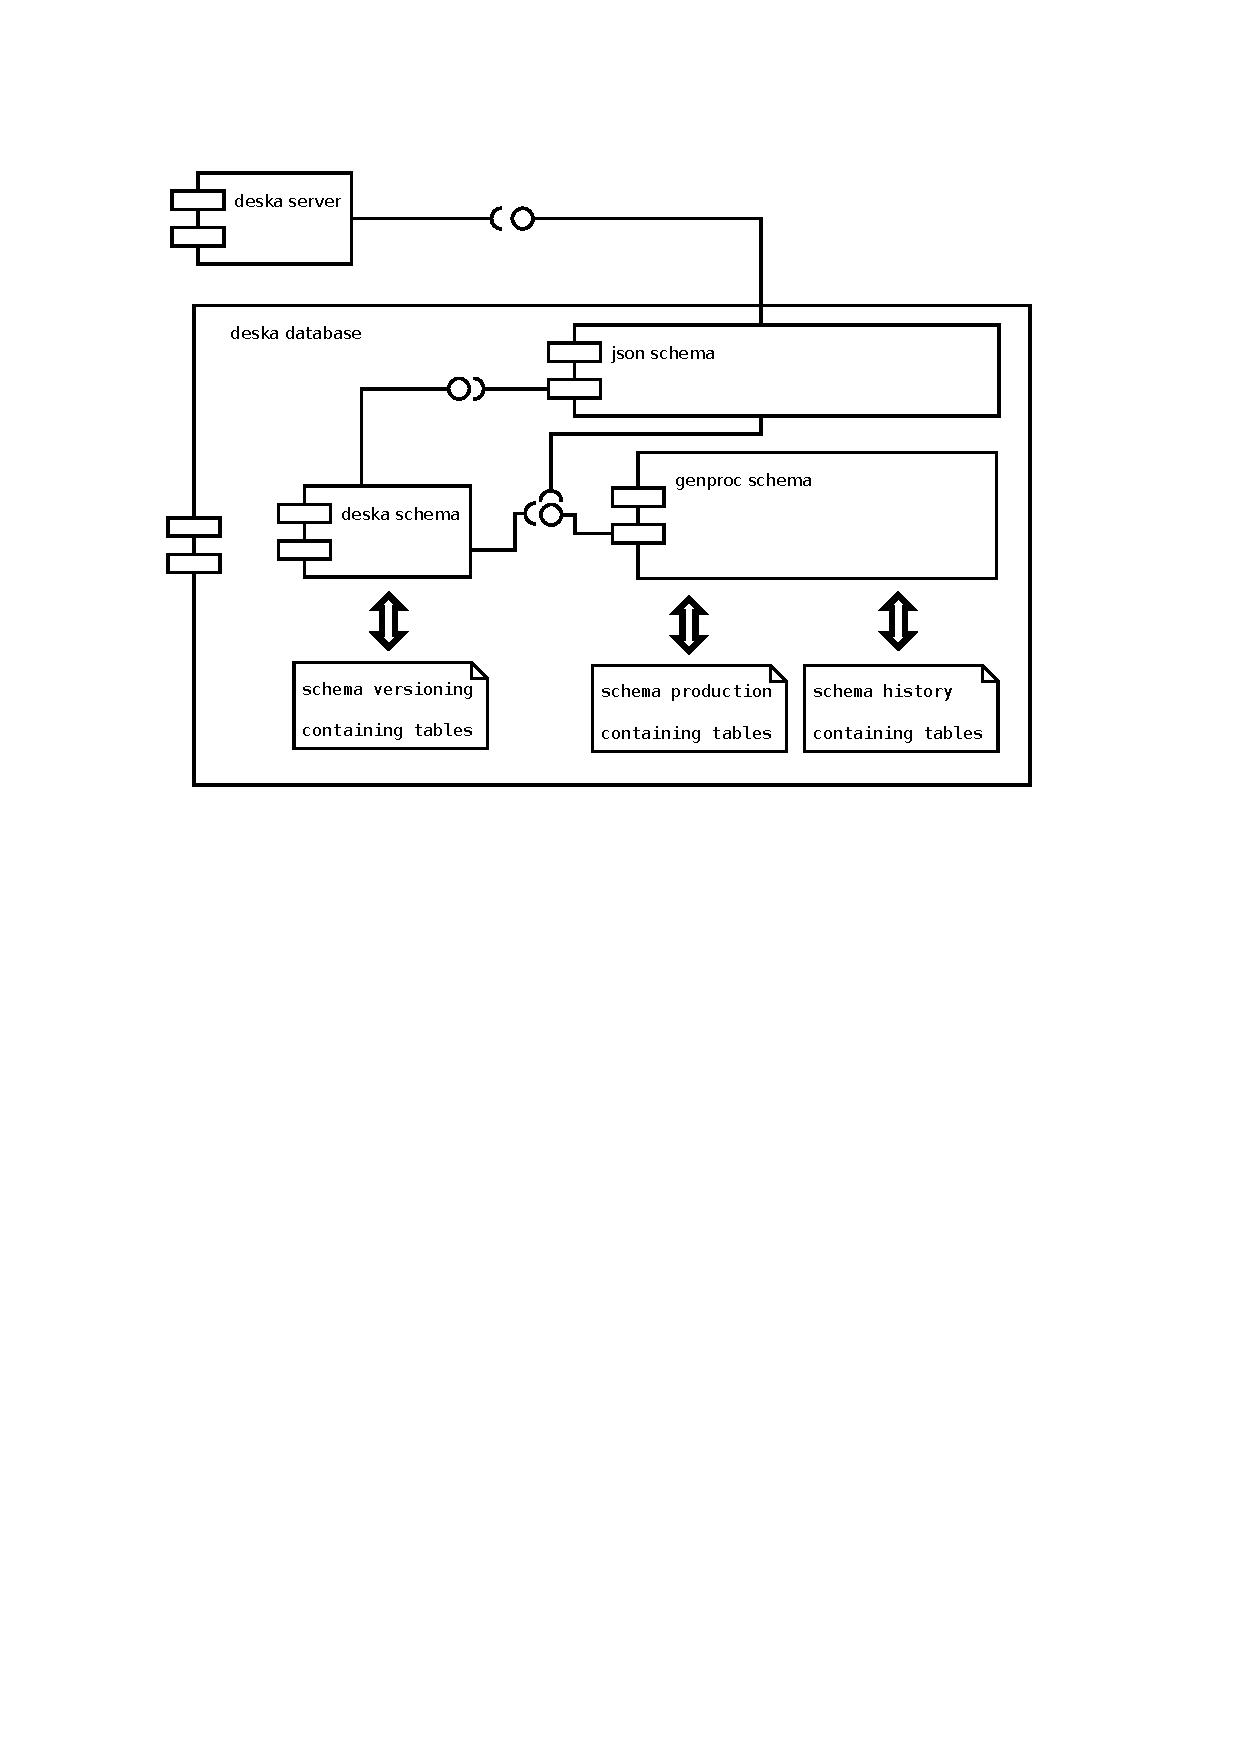
\includegraphics[trim=28mm 170mm 30mm 28mm]{img-deska-server-components.pdf}
	\caption{Deska server components}
\end{figure}

All communication with Deska server is implemented in schema json. There are functions, written in pg-python, which use another
functions, to manipulate with data in database. Or get data directly from tables as in {\tt pendingChangeset} and {\tt listRevisions}
\footnote{This direct access is not shown in the picture}.
Why we created this layer, and why it returns JSON data and not table or normal value, will be described in \secref{sec:schema-json}

The picture \ref{img:deska-server} shows how Deska server and Deska database communicate. Schema json provides interface for Deska server. It
calls functions from other schemas (genproc and Deska). All these schemas are drawn as components. Schemas containing
tables are shown in different form, because they do not provide real interface.

\subsection{Json schema}
\label{sec:schema-json}
After we had generated functions for manipulating with data, and DBAPI specified, it was clear, that there must be some layer,
that transforms createObject(kindName,xxx) to kindName\_add(xxx), which is call of generated SQL function.
We do that in Deska database, because we wanted to have 1:1 mapping between database functions, and DBAPI commands.

It worked well until first performance testing was made. The state was, that Deska server call for data - millions of objects,
database worked and worked and... when finally returned this data to server, server started transformation... It took long time
and consumed lots of memory.
In the same time, diffing implementation started, and there where problems with many functions of different result types,
that has to be called, which was hard to union into one function.
So there was an idea, that JSON can be created inside database, so that the union of diffing function can return JSON.

Some test were run \secref{sec:test-json}, the time for smaller data was worse with JSON in database, but for large data, there was significant
speed up. The function written in pg-python creates part of the JSON structure in each line of database cursor.
So the JSON structure grows up with data that database produced.

The result is, that every function callable by server returns JSON.

\subsection{Getting data from tables}
\label{sec:data-functions}
Here we talk about getting data of objects, revisions and changesets stored in tables.
These data are get from tables, or table returning functions for get data in proper version.
See \secref{sec:versioning} how these functions works. Here we talk about functions in json schema.

There are {\tt pendingChangeset} that selects data from changeset table, and {\tt listRevisions} that selects data from version table.
Both accept filter as parameter and uses some cast optimization, about which we will talk in section about cast
optimization \secref{sec:cast}.

Object data functions {\tt objectData}. {\tt resolvedObjectData}. {\tt resolvedObjectDataWithOrigin} calls generated functions 
that returns tuple of attribute values, that is just converted into JSON format and returned. 

In functions {\tt multipleObjectData}. {\tt multipleResolvedObjectData} and {\tt multipleResolvedObjectDataWithOrigin}
more work is done, than in another json schema function, that only runs some function.
There is still only one main call another database function (and one helping, to get revision number).

But the SQL statement to run is created in more difficult way. In contrast to other json schema functions,
here we create complicated {\em column definition} for the SQL statement. It goes between SELECT and FROM keywords.
This column definition contains definition of all columns that shall be returned in human readable form.
In database tables, reference columns has bigint type, but user wants to see text name of referenced kind.
The sets are represented by another table, but user wants to see array etc. So some transformation must be done.
It is the easiest for simple attribute,
for example if kind host has attribute note, than the column definition is {\em host.note}.
It gets complicated, when the attribute is part of some relation. For example refers\_to.
If host has attribute hardware, referencing to kind hardware. Than column definition is 
{\em hardware\_get\_name(host.hardware,\$1)}. For sets, templates and embed kinds it is similar.

\subsubsection{Example}
Lets see the {\tt multipleResolvedObjectDataWithOrigin} function to explain, how it work. The other functions are very similar.
At first, name is set (this is used for result JSON and/or reporting errors) and JSON structure is prepared,
using dutil.jsn function. After this, kindName is checked. Then attributes are load from generated.py file.
If kind has template, every attribute except one starts with template\_ prefix are duplicated, so that we has
also information about origin of the value.
Then columns definition is generated. For normal attribute, "kindName.attributeName" is the definition.
But for referenced attributes, which are
represented as uid in database, not string, kindName\_get\_name function must be called. So in the case that attribute vendor is represented as id, then
"vendor\_get\_name(kindName.attributeName, version) AS kindName.attributeName" is the column definition. For embedded kind, embed name is created in similar way,
using function join\_with\_delim.
Then, the final SQL statement is created using function dutil.getSelect, columns definition and JOIN and WHERE parts from filter are used.
This function also checks if this kind has template or not, and proper function resolved or not is used in the final SQL statement.

After this preparation, SQL statement is run and the result is fetched. For each line in the result table, one part of result JSON structure is
created. And then final JSON is created and returned.

And here is some example of SQL statement which is called:
\begin{minted}{sql}
SELECT host.service_templ --simple column definition
,host.name,host.service,host.virtual_hardware_templ,
host_template_get_name(host.template_host,$1) AS host_template --column definition for uid column of template
,hardware_get_name(host.hardware,$1) AS hardware, --column definition for uid column of reference
host.note_host_templ,virtual_hardware_get_name(host.virtual_hardware,$1) AS virtual_hardware,
host.hardware_templ,
host.note_host FROM
host_resolved_data_template_info($1) AS host -- call function for get resolved data with template info
LEFT OUTER JOIN hardware_resolved_data($1) AS hardware ON host.uid = hardware.host -- join host kind
WHERE hardware.name != $2 OR hardware.name IS NULL -- perform filter condition
\end{minted}

\subsection{Direct access to resolved data}
\label{sec:direct-access}
If you are not in changeset, and do not give revision parameter to function {\tt multipleResolvedObjectData},
you will access directly, because resolved data are in production schema tables.

This is used by configuration generators and it is much more faster to read
resolved data than do this in history schema, where compilated computation is run.
See test results in \secref{sec:test-direct}

\subsection{Getting data from tables - casting}
\label{sec:cast}
For performance reasons we do one more thing in column definition. It is casting.
In pg-python extension, there is some function that from Postgresql types create native python types.
It is called Postgres.convert\_postgres\_objects
and must be called for every result from database. But it supports only some types.
Some of these types are converted in different way than we want.

At first, we solved this with our own function, that did the transformation, but if it ran for every
row and every column, it was very slow. So the most of these transformations is now done using Postgresql cast
in SQL statements. It is much faster and saves memmory (see \secref{sec:test-cast}

The column definition is more complicated than we describe above. If
Postgres.convert\_postgres\_objects function 
does not support conversion of given column's type, or do it in bad way for us, we add cast in column definition.
For example if there is timestamp attribute, we add {\em ::text}, if it is ipv4 type, and we don't want
the conversion with mask suffix, we use {\em host} function in column definition.


\subsection{Filters}

Some functions (lets call them {\em data functions} in json schema have parameter filter. It is in JSON format,
see DBAPI protocol in~\secref{sec:api-filters} for more info.
The data function, in json schema, have part where SQL statement is created. It is described in
\secref{sec:data-functions}.

This filter is implemented in filter.py file in class {\tt Filter}.
It adds JOIN and WHERE parts to the SQL statement that is used by data functions. The {\tt Filter} class has
methods getJoin and getWhere that return strings which fit at the end of SQL statement in data function.

Filter constructor parses given filter into parts - conditions.
Every condition has kind, attribute, operator and value. From this we create strings line
{\em kind.attribute = kind2\_get\_uid(\$2)}. If there are more conditions, they are joined with AND or OR
operators.
If kind in condition is different from kindName - function parameter, it is remember,
and in getJoin function, if it is possible, string like {\em JOIN kind2 ON kind2.uid = kind.attribute}
is returned. This is possible when some relation between this kinds exists.
If there are more different kinds, join string with more JOINs is produced.
Information about relation are taken from generated.py file.

It was add into Deska later than other functions, so that it uses what was developed before.

\subsection{Filters limitations}
\label{sec:filter-speed}
As we have said, filtering requirement was add very late. In that time, data functions has parameter revision
and only way to implement this is via function returning table.

So the filter is applied on the result of this function, providing parametrized view.
Except in {\em multipleResolvedObjectData}, which access directly to the tables, when
you are not in changeset and revision parameter is not set.

But main problem is not, what to select at first. It is that table returning function has
no indexes and every filtering is done by full table scan.
This slows filters down, and it must be improved in the future. It is not hard,
if you use view instead of function simulating parametrized view, indexes can be used.
And as we can see, revision parameter is not used now, so if DBAPI specification changes,
we can transform this functions into views. 

\subsection{Error handling}
Here we try to explain work with exceptions in Deska database and Deska server. Postgresql functions can RAISE exception with given message and sqlstate.
This sqlstate is like number of error. We use this to split possible exceptions into some categories - exception types. Exception in database is
every unexpected or “bad” thing that occurs. It can be runtime error as well as constraint violation, or exception thrown explicitly by RAISE.

While json schema provides JSON as return type, we try to catch maximum number of exception inside the database (in
json schema part).
For this catching DeskaException class is used. It has constructor, with Postgresql.dberr as parameter, which structure is that contains exception
message, and sqlstate. We use this information to determine exception type - class contains typeDict - dictionary {sqlstate: exceptionType}.
Finally this function has {\tt json} method, which takes name on the function, in which error occurs and creates exception in JSON format.

\label{sec:deska-db}

In this section you can find how the Deska db works, how the data versioning, templating and other deska's features are done.\\
Almost all tables and stored procedures are generated by sql-generator described in \secref{sec:sql-generator}.

\section{Data manipulation in Deska database}
\label{sec:deska-db-data-manipulation}
Here you can find how the Deska database works, how the data versioning, templating and other Deska's features are done.

\subsection{Versioning}
\label{sec:versioning}

\todo{About changeset/version tables and functions around}

The database can return object's data in any version in which it exists. This could be done due to history tables that are generated for each table defined by user.\\
Each history table contains, in addition to attributes in the table defined by user, attributes {\tt version} and {\tt dest\_bit}. In version attribute is information about the changeset in which the object was modified. {\tt dest\_bit} attribute set to 1 means that the object is deleted, default value is 0.\\

\subsubsection{Data Modification}

\begin{longtable}{ l | l | l | l | l | l }
    \caption{Database table {\tt hardware\_history}}
    \label{tab:example-hardwarehist} \\
    name & uid & purchase & note & dest\_bit & version\\
    \hline
    \endhead
    h1 & 1 & & & 0 & 1 \\
    h2 & 2 & & & 0 & 1 \\
    h2 & 2 & & note & 0 & 2 \\
    h2 & 2 & 01-01-2011 & note & 0 & 3 \\
    h1 & 2 & & & 1 & 3 \\
    \hline
\end{longtable}

In table \ref{tab:example-hardwarehist} is example of hardware's history table. This is how the hardware\_history table looks like after following operations. 
\begin{itemize}
    \item In changeset 1 were inserted hardware h1, h2.
    \item In changeset 2 was h2's note attribute set to note.
    \item In changeset 3 was h2's purchase attribute set to 01-01-2011 and hardware h1 was deleted.
\end{itemize}


If the table \ref{tab:example-hardwarehist} was only a piece of data from hardware\_history table then we could not recognize if these objects were in changeset 1 created or some of their attributes were just set.\\
In row with hardware h2, version 3 we can see that when object is modified, row with its actual data and id of current changeset is inserted into history table, after that the attribute which has to be modified is set.\\
In words of stored procedures it could be written so:\\

\begin{minted}{sql}
select startchangeset();
select hardware_add('h1');
select hardware_add('h2');
select commitchangeset('.');

select startchangeset();
select hardware_set_note('h2','note');
select commitchangeset('.');

select startchangeset();
select hardware_set_purchase('h2','01-01-2011');
select hardware_del('h1');
select commitchangeset('.');
\end{minted}

\subsubsection{Retrieve Object Data}

If we would like to get data of some objects in given version. We have to find the objects' last modification. To find the really last objects' modification, we need to know version table.\\
At the time of changeset commit, table with versions is updated. For our example it could looks like \ref{tab:example-version}.\\
Important information for us are id and num. id is id of changeset from which the version num was created. The version number num is an increasing sequence, if version num2 was created on the base of version num1 then num1 < num2.


\begin{longtable}{ l | l | l | l | l }
    \caption{Database table {\tt version}}
    \label{tab:example-version} \\
    id & num & author & timestamp & message\\
    \hline
    \endhead
    0 & 1 & martina & 2011-12-17 17:04:29.56794 & Initial revision\\
    1 & 2 & martina & 2011-12-17 17:04:47.876152 & .\\
    2 & 3 & martina & 2011-12-17 17:04:54.731837 & .\\
    3 & 4 & martina & 2011-12-17 17:05:12.489788 & .\\
    \hline
\end{longtable}


There are some examples of data retrieving, results are in table \ref{tab:select-hardware} and table \ref{tab:select-hardware-v3}.\\

\begin{minted}{sql}
--functions for data retrieving without parameters returns the most actual data
select * from hardware_data_version();
select * from hardware_data_version(3);
\end{minted}

\begin{longtable}{ l | l | l | l | l | l }
    \caption{Database table {\tt hardware\_data\_version()}}
    \label{tab:select-hardware} \\
    uid & name & note & purchase & version & dest\_bit\\
    \hline
    \endhead
    2 & h2 & note & 2011-01-01 & 3 & 0\\
    \hline
\end{longtable}

\label{tab:select-hardware-v3}
\begin{longtable}{ l | l | l | l | l | l }
    \caption{Database table {\tt hardware\_data\_version(3)}} \\
    uid & name & note & purchase & version & dest\_bit\\
    \hline
    \endhead
    1 & h1 &  &  & 1 & 0\\
    2 & h2 & note &  & 2 & 0\\
    \hline
\end{longtable}

\subsubsection{Commit}
Commit function selects objects from history table of given kind which were just added, deleted or updated in the current changeset. Rows that belong to added objects are inserted into given kind's table in the schema production. Rows that belong to deleted objects are deleted from kind's table in the schema production. And rows that belong to updated objects are updated in kind's table in the schema production.\\
Commits from our example will cause these changes:
\begin{itemize}
    \item After changeset 1 rows with hardware h1, h2 will be inserted.
    \item After changeset 2 h2's note attribute will be updated.
    \item After changeset 3 h2's purchase attribute will be updated and hardware h1 will be deleted.
\end{itemize}

\subsection{Refers To}
\label{sec:db-refs-to}
If the table is in the {\tt REFERS TO} relation with another, it has to have column that refers to the {\tt uid} column of the another table. This column, which refers to the {\tt uid} column of another table, we will call here {\em refuid}.\\
Stored procedures for setting refuid columns expect as parameter some value of name attribute from referenced table. The given name is found in referenced table and proper {\tt uid} is set as value of refuid column instead of the name.

Here is an example of setting refuid column. The result of these selects is in tables \ref{tab:refs-hardware} and  \ref{tab:refs-vendor}.
\begin{minted}{sql}
select startchangeset();
select vendor_add('v1');
select vendor_add('v2');
select hardware_add('h1');
select hardware_set_vendor('h1','v2');
select commitchangeset('.');

select * from hardware;
select * from vendor;
\end{minted}

\begin{longtable}{ l | l | l | l | l }
    \caption{Database table {\tt hardware}}
    \label{tab:refs-hardware} \\
    uid & name & note & purchase & vendor\\
    \hline
    \endhead
    1 & h1 &  &  & 2\\
    \hline
\end{longtable}

\begin{longtable}{ l | l }
    \caption{Database table {\tt vendor}}
    \label{tab:refs-vendor} \\
    uid & name \\
    \hline
    \endhead
    1 & v1\\
    2 & v2\\
    \hline
\end{longtable}


\subsection{Object Embedding}
Object embedding is described in \ref{sec:relation-embed-into}. The object which is embedded into another object could be identified by the global name, pair of object's local name and parent's name. Embedded objects have an attribute which refer to the parent object's uid. With this attribute is manipulated in the same way as with the refuid attributes described in \ref{sec:db-refs-to}.\\
The following example shows how to work with embedding, the table identifier is embedded into the table host. Result of these selects is in the tables \ref{tab:embed-host} and \ref{tab:embed-interface}.

\begin{minted}{sql}
select startchangeset();
select host_add('h1');
select host_add('h2');
select interface_add('h1->i1');
select interface_add('h1->i2');
select interface_add('h2->i1');
select commitchangeset('r2');
\end{minted}


\begin{longtable}{ l | l }
    \caption{Database table {\tt host}}
    \label{tab:embed-host} \\
    uid & name \\
    \hline
    \endhead
    1 & h1\\
    2 & h2\\
    \hline
\end{longtable}

\begin{longtable}{ l | l | l | l }
    \caption{Database table {\tt interface}}
    \label{tab:embed-interface} \\
    uid & name & host & note\\
    \hline
    \endhead
    1 & i1 & 1 & \\
    2 & i2 & 1 & \\
    3 & i1 & 2 & \\
    \hline
\end{longtable}


\subsection{Templates}
{\tt TEMPLATIZED} relation which is described in \ref{sec:relation-templatized} is implemented by template tables. 

\subsubsection{Value inheritance}
The columns, which are a part of some {\tt COMPOSITION} relation or {\tt EMBED INTO} relation, can not inherit its value from templates. Therefore these columns are not present in the template table. All other attributes from the templated table are also in the template table.\\
As the template tables are templated by themself, object can inherit value of its attributes transitively from more templates.\\
To ensure right data retrieving from given version, template tables need to have history tables as well.\\
Tables in the schema production store resolved data.\\
The following example shows how we can work with the templated tables. The hardware table is templated by the hardware\_template table. The result of these selects is in tables \ref{tab:templ-hwhist} and \ref{tab:templ-hwtemplhist}.

\begin{minted}{sql}
select startchangeset();
select hardware_template_add('t1');
select hardware_template_set_note('t1','note from template t1');
select hardware_template_set_purchase('t1','01-01-2011');
select hardware_add('h1');
select hardware_set_template_hw('h1','t1');
select commitchangeset('r2');

select startchangeset();
select vendor_add('v1');
select hardware_template_add('t2');
select hardware_template_set_vendor('t2','v1');
select hardware_template_set_purchase('t2','01-01-2011');
select hardware_template_set_template_hw('t1','t2');
select commitchangeset('r3');

select startchangeset();
select hardware_set_note('h1','own h1 note');
select commitchangeset('r4');
\end{minted}


\begin{longtable}{ l | l | l | l | l | l | l | l }
    \caption{Database table {\tt hardware\_history}}
    \label{tab:templ-hwhist} \\
    uid & name & note & purchase & vendor & template\_hw & version & dest\_bit\\
    \hline
    \endhead
    1 & h1 &  &  &  & 1 & 1 & 0\\
    1 & h1 & own h1 note &  &  & 1 & 3 & 0\\
    \hline
\end{longtable}

\begin{longtable}{ l | l | l | l | l | l | l | l }
    \caption{Database table {\tt hardware\_template\_history}}
    \label{tab:templ-hwtemplhist} \\
    uid & name & note & purchase & vendor & template\_hw & version & dest\_bit\\
    \hline
    \endhead
    1 & t1 & note from template t1 & 2011-01-01 &  &  & 1 & 0\\
    2 & t2 &  & 2011-01-01 & 1 &  & 2 & 0\\
    1 & t1 & note from template t1 & 2011-01-01 &  & 2 & 2 & 0\\
    \hline
\end{longtable}


By calling the following commands we can get resolved data, it means with inherited values.\\
It is possible to get resolved data even with the data origin, this function is introduced in subsection about multi-value references \ref{sec:multi-val}.
\begin{minted}{sql}
--from version 'r3'
select * from hardware_resolved_data(3);
select * from hardware_template_resolved_data(3);
\end{minted}

Results are in \ref{tab:templ-hwres2} and \ref{tab:templ-hwtemplres2}.

\begin{minted}{sql}
--in production are the newest resolved data
select * from hardware;
select * from hardware_template;
\end{minted}
Results are in \ref{tab:templ-hw} and \ref{tab:templ-hwtempl}.

\begin{longtable}{ l | l | l | l | l | l | l }
    \caption{Database table {\tt hardware\_resolved\_data(3)}}
    \label{tab:templ-hwres2} \\
    uid & name & note & purchase & vendor & template\_hw & dest\_bit\\
    \hline
    \endhead
    h1 & 1 & note from template t1 & 2011-01-01 & 1 & 1 & 0\\
    \hline
\end{longtable}

\begin{longtable}{ l | l | l | l | l | l | l }
    \caption{Database table \\ {\tt hardware\_template\_resolved\_data(3)}}
    \label{tab:templ-hwtemplres2} \\
    uid & name & note & purchase & vendor & template\_hw & dest\_bit\\
    \hline
    \endhead
    t2 & 2 &  & 2011-01-01 & 1 &  & 0\\
    t1 & 1 & note from template t1 & 2011-01-01 & 1 & 2 & 0\\
    \hline
\end{longtable}

\begin{longtable}{ l | l | l | l | l | l }
    \caption{Database table {\tt hardware}}
    \label{tab:templ-hw} \\
    uid & name & note & purchase & vendor & template\_hw\\
    \hline
    \endhead
    1 & h1 & own h1 note & 2011-01-01 & 1 & 1\\
    \hline
\end{longtable}

\begin{longtable}{ l | l | l | l | l | l }
    \caption{Database table {\tt hardware\_template}}
    \label{tab:templ-hwtempl} \\
    uid & name & note & purchase & vendor & template\_hw\\
    \hline
    \endhead
    1 & t1 & note from template t1 & 2011-01-01 & 1 & 2\\
    2 & t2 &  & 2011-01-01 & 1 & \\
    \hline
\end{longtable}

\subsubsection{Commit of Templated Tables}
As data in the production schema are resolved, it is needed during commit find modified objects and resolve their data. We should keep in mind that object's data could be modified even by modification in the object that templates this object.\\
Commit of templated table is composed of:
\begin{enumerate}
    \item find all objects in the template table that were modified in the current changeset
    \item find all objects in the template table that can transitively inherit data from objects in step 1
    \item find all objects in the templated table that inherit data from objects in step 2
    \item resolve data of objects from step 3
    \item process data from step 4 as it was selected from history table of not templated table
\end{enumerate}

\subsection{Diff}
Modifications which were done between two versions or inside a temporary changeset could be listed by diff functions. Diff has these stages:
\begin{enumerate}
    \item init diff
    \item process diff data
    \item terminate diff
\end{enumerate}
Stage init diff creates temporary table with almost all data needed to get list of all modifications.
More init functions exist, one for diff between two versions and one for diff between state in temporary changeset and in its parent version. For templated kinds these init diff functions exist even in resolved modification.\\
Temporary table created in init diff stage could be then processed by diff functions. Each type of "basic modification" described in DBAPI \ref{sec:dbapi-protocol} is listed by separate diff function. Basic modifications setting a single attribute are listed by one function for all attributes of {\tt identifier\_set} type and next one for the rest of attributes.\\
The example below shows how you can select changes between versions.

\begin{minted}{sql}
select startchangeset();
select hardware_add('h1');
select hardware_add('h2');
select hardware_set_purchase('h1','02-12-2011');
select commitchangeset('r2');

select startchangeset();
select hardware_set_purchase('h1','01-01-2012');
select hardware_add('h3');
select hardware_del('h2');
select hardware_set_name('h1','hr');
select commitchangeset('r3');

--init
select hardware_init_diff(2,3);

--process diff data
select * from hardware_diff_created();
--returns h3

select * from hardware_diff_deleted();
--returns h2

select * from hardware_diff_rename();
--returns oldname:h1   newname:hr

select * from hardware_diff_set_attributes(2,3);
--returns objname:hr   attribute:purchase   olddata:2011-02-12   newdata:2012-01-01

--terminate
select hardware_terminate_diff();
\end{minted}

\subsection{Composition}
Composition is described in \ref{sec:relation-contains}.
Linking objects with the same name from different tables is maintained by before and after insert and update triggers. These triggers ensure even disjoining if one of linked objects is renamed or deleted and can immediately join renamed object with another one.\\
Condition that one object could be contained in at most one another object is checked by the check constraints. When the table represents kind that is containable to more than one kind, the containable table has this check constraint.\\
Following example shows, how the objects in {\tt COMPOSITION} relation are linked and disjoint. Result is in tables \ref{tab:comp-box}, \ref{tab:comp-hw} and \ref{tab:comp-switch}.

\begin{minted}{sql}
select startchangeset();
select hardware_add('h1');
select hardware_add('h2');
select hardware_add('h3');
select box_add('h1');
select box_add('h3');

--select switch_add('h1');
--would raise exception (violates check constraint) - h1 switch and h1 hardware can not contain the same box
select box_add('o1');
select commitchangeset('r2');

select startchangeset();
--renamed hardware is immediately linked with box with the same name
select hardware_set_name('h2','o1');
select hardware_del('h3');
--box h3 is now free, switch h3 could containt box h3
select switch_add('h3');
select commitchangeset('r3');

select uid, name, box from hardware;
select uid, name, hardware, switch from box;
select uid, name, box from switch;
\end{minted}

\begin{longtable}{ l | l | l | l }
    \caption{Database table {\tt box}}
    \label{tab:comp-box} \\
    uid & name & hardware & switch\\
    \hline
    \endhead
    1 & h1 & 1 & \\
    3 & o1 & 2 & \\
    2 & h3 &  & 1\\
    \hline
\end{longtable}

\begin{longtable}{ l | l | l }
    \caption{Database table {\tt hardware}}
    \label{tab:comp-hw} \\
    uid & name & box\\
    \hline
    \endhead
    1 & h1 & 1\\
    2 & o1 & 3\\
    \hline
\end{longtable}

\begin{longtable}{ l | l | l }
    \caption{Database table {\tt switch}}
    \label{tab:comp-switch} \\
    uid & name & box\\
    \hline
    \endhead
    1 & h3 & 2\\
    \hline
\end{longtable}


\subsection{Multi-value References}
\label{sec:multi-val}
Multi-value references are described in \ref{sec:relation-multi-value-references}.\\
For each table's attribute, which is a part of some multi-value reference, is generated table, we call it {\em inner table}. This inner table stores for each object from the table its {\tt identifier\_set} value.\\

\subsubsection{Data Modifications and Versioning}
As inner table stores data of attribute that is part of versioned data, it is needed to have history table for all inner tables as well.\\ 
In addition to ordinary set attribute functions {\tt identifier\_set} attributes could be modified also by functions that insert or remove identifier into or from identifier set.\\
Each inner table has attribute flag that is used to distinguish between rows representing empty set from rows representing NULL value.\\
Following example shows how we can work with {\tt identifier\_set}s. In tables \ref{tab:multi-hosthist} and \ref{tab:multi-innerhist} you can see whole history of objects in the example. The table \ref{tab:multi-hostv} shows result of the last select, it selects data from given version.

\begin{minted}{sql}
select startchangeset();
select service_add('s1');
select service_add('s2');
select service_add('s3');
select host_add('h1');
select host_add('h2');
select host_set_service('h1',ARRAY['s1','s2']);
select commitchangeset('r2');

select startchangeset();
--we can remove just one item from identifier_set
select host_set_service_remove('h1','s2');
--we can insert just one item to identifier_set
select host_set_service_insert('h2','s3');
select commitchangeset('r3');

select startchangeset();
--host h1 has now empty set of services
--flag is still 1
select host_set_service_remove('h1','s1');
select commitchangeset('r4');

select startchangeset();
--flag is now 0
select host_set_service('h1',NULL);
select commitchangeset('r5');

select * from host_history;
select * from inner_host_service_history;
--this is how you can get hosts' services in given version
select uid, name, host_get_service(uid,4) from host_data_version(4);
\end{minted}

\begin{longtable}{ l | l | l | l }
    \caption{Database table {\tt host\_history}}
    \label{tab:multi-hosthist} \\
    uid & name & dest\_bit & version\\
    \hline
    \endhead
    1 & h1 & 0 & 1\\
    2 & h2 & 0 & 1\\
    1 & h1 & 0 & 2\\
    2 & h2 & 0 & 2\\
    1 & h1 & 0 & 3\\
    1 & h1 & 0 & 4\\
    \hline
\end{longtable}

\label{tab:multi-innerhist}
\begin{longtable}{ l | l | l | l }
    \caption{Database table {\tt inner\_host\_service\_history}} \\
    host & service & flag & version\\
    \hline
    \endhead
    1 & 1 & 1 & 1\\
    1 & 2 & 1 & 1\\
    1 & 1 & 1 & 2\\
    2 & 3 & 1 & 2\\
    1 &  & 1 & 3\\
    1 &  & 0 & 4\\
    \hline
\end{longtable}

\begin{longtable}{ l | l | l }
    \caption{Database table {\tt host}}
    \label{tab:multi-hostv} \\
    uid & name & service\\
    \hline
    \endhead
    1 & h1 & \{\}\\
    2 & h2 & \{s3\}\\
    \hline
\end{longtable}

\subsubsection{Templates}
The table, to which attribute an inner table is made, could also be templated. So it is needed to have template table of these inner tables and have functions for resolving templated inner table's data.\\
Following example shows how we can work with templated {\tt identifier\_set}s. Promised example of function, which retrieves resolved objects' data with the data origin, is introduced in the example. Also the function which process diff data and lists data modifications of {\tt identifier\_set} attributes is showed in the example.\\

\begin{minted}{sql}
select startchangeset();
select service_add('s1');
select service_add('s2');
select service_add('s3');
select host_add('h1');
select host_add('h2');
select host_template_add('t1');
select host_template_add('t2');
select host_template_set_service('t2',ARRAY['s1','s2']);
select host_template_set_template_host('t1','t2');
select host_template_set_note_host('t1','note from t1');
select host_set_template_host('h1','t1');
select host_set_template_host('h2','t2');
select commitchangeset('r2');

select startchangeset();
select host_set_service_remove('h2','s2');
select host_template_set_service_insert('t1','s3');
select commitchangeset('r3');

select host_init_resolved_diff(2,3);
select * from host_diff_refs_set_set_attributes(2,3);
--returns these two rows
--objname:h1 attribute:service olddata:{s1,s2} newdata:{s1,s2,s3}
--objname:h2 attribute:service olddata:{s1,s2} newdata:{s1}

select host_terminate_diff();
\end{minted}

By calling the following selects we can get resolved data with the data origin, it means with inherited values and name of the object from which was the value taken.\\
\begin{minted}{sql}
select * from host_resolved_data_template_info();
select * from host_resolved_data_template_info(2);
\end{minted}

Results are in tables \ref{tab:multi-reshost} and \ref{tab:multi-reshostv2}.

\begin{longtable}{ l | l | l | l | l | l | l }
    \caption{Database table {\tt host\_resolved\_data\_template\_info()}}
    \label{tab:multi-reshost} \\
    uid &  name &  service &  service\_templ &  note\_host &  note\_host\_templ &  template\_host\\
    \hline
    \endhead
    2 & h2 & \{s1\} & h2 &  &  & 2\\
    1 & h1 & \{s1,s2,s3\} & t1 & note from t1 & t1 & 1\\
    \hline
\end{longtable}

\begin{longtable}{ l | l | l | l | l | l | l }
    \caption{Database table {\tt host\_resolved\_data\_template\_info(2)}}
    \label{tab:multi-reshostv2} \\
    uid &  name &  service &  service\_templ &  note\_host &  note\_host\_templ &  template\_host\\
    \hline
    \endhead
    2 & h2 & \{s1,s2\} & t2 &  &  & 2\\
    1 & h1 & \{s1,s2\} & t2 & note from t1 & t1 & 1\\
    \hline
\end{longtable}



\label{sec:sql-procedures}

\section{SQL generator}
\label{sec:sql-generator}
This section describes how the tables and functions in the Deska database are generated. The Deska database is described in \secref{sec:deska-db}.\\
The SQL generator is run by Deska database intstallator. It generates stored procedures and tables that ensure data manipulation for scheme described by user in module tables.\\

The generator is composed of classes {\tt Connection}, {\tt Schema}, {\tt Table}, {\tt Template}, {\tt Composition} and {\tt Multiref}.\\
The significant part of each class are string constants that represent plpgsql code with mapping keys. These string constants are formatted in class methods, mapping keys are replaced with appropriate parts of plpgsql code that could differ for various tables.
Detailed information about mentioned classes are below.

Parts of plpgsql generator run at the moment when all modules defined by user are already present as tables in the database. And they start in this order:

\begin{enumerate}
    \item {\tt Template} class - generate and create templates for tables that should have template
    \item {\tt Schema} class, {\tt Table} class - generate and create history tables for all tables (even for template tables that were generated)
    \item {\tt Schema} class, {\tt Table} class - generate and create stored procedures for data manipulation (the same stored procedures for tables defined by user and template tables)
    \item {\tt Multiref} class - generate and create tables and stored procedures for {\tt identifier\_set}s, history and template table for {\tt identifier\_set}s.
    \item {\tt Composition} class - generate and add triggers for {\tt COMPOSITION} relation
\end{enumerate}

\subsection{Schema}
The {\tt Schema} class controls generation of plpgsql code for creation of data manipulation functions. It is instantiated with {\tt Connection} parameter, which is used to query the database. 
The {\tt Schema} class finds out which kinds were created in database and what their structure is. The {\tt Schema} class instantiates {\tt Table} classes one by one for each kind defined by user. Appropriate methods of {\tt Table} class that generate plpgsql code according to kind's characteristics are then called.\\ It is necessary to distinguish between kinds that are {\tt EMBED INTO} (see \secref{sec:relation-embed-into}) and that are not. The part of data manipulation functions, where the concrete objects are identified and selected should be different for those {\tt EMBED INTO} and those not {\tt EMBED INTO} kinds.
For {\tt templated} kinds (\secref{sec:relation-templatized}) are in addition to not templated kinds generated functions for getting resolved data.\\
The final code for created kinds is generated inside the {\tt Table} class.

\subsection{Table}
A lot of string constants are present inside the {\tt Table} class. These string constants are prototypes of create tablem, create type statements, create function statements or some other pieces of plpgsql code.\\
Methods of {\tt Table} class return concrete plpgsql code for creating history tables and data manipulation functions. Generated functions are prepared to be created on the database server.\\

\begin{enumerate}
    \item get data functions
    \item add, delete objects, set attribute functions
    \item diff functions
    \item commit
\end{enumerate}

\subsubsection{History tables}
In following text we will talk about {\tt table} and its history table {\tt table\_history}.\\
For each table created in schema production a table with suffix \_history is generated. {\tt table\_history} serves as complete history of objects of kind that is represented by {\tt table} in database. These history tables are created in schema history.\\
{\tt table\_history} has the same attributes like {\tt table} and in addition {\tt dest\_bit} and {\tt version} attributes. {\tt dest\_bit} attribute indicates whether the object was deleted or not. In {\tt version} attribute is stored in which changeset was this row inserted. Inserted rows represents new object creation but even modification of an object. Don't confuse this {\tt version} attribute with the number of revision.

\subsubsection{Retrieve Object Data}
Getting objects' data means getting data of these objects' last modification before the given version in which user would like to get them.
In resolved modifications (resolving inherited values from object templates) of get data functions it is needed to resolve these data. And to resolve them again use inherited data from templates' last modification before the given version.
These resolving functions are written as recursive selects.

\subsubsection{Performing Modifications}
Create new object is done by inserting a row with values given {\tt name}, {\tt uid}, {\tt dest\_bit} set off and id of current changeset in {\tt version} attribute into history table.\\
Set attribute operation inserts current data of the object which we would like to modify into history table, sets value of version attribute to id of current changeset and updates the value of attribute, which has to be set.\\
Object deletion is done by setting {\tt dest\_bit} attribute on.\\
The {\tt dest\_bit} attribute can be also set from on to off, this is the way, how we can undo deletion. But it is enabled only in the same changeset in which it was set to on. This deleted object will not exist later and will not be found.

\subsubsection{Diff}
For diffing are generated functions for diff initialization, processing data prepared during the initialization and cleaning after diff. For templated tables is generated also the resolved modification of function for diff initialization. Data processing stays the same even for diff of resolved data, because all data resolving is done in the initialization step.\\
These diff initialization functions have two other forms, for getting list of modifications between two versions and between the state inside temporary changeset and in its parent version. Even data processing have to take into consideration between which stages is diffing done. It is because it is needed for columns, which refers to some table uid and were changed, the proper name have to be taken.

\subsubsection{Commit}
Table class for given table generates also commit function that bring tables in the production schema up to data. As data in tables in the production schema are resolved and templated data could be modified even by a change in the template table, it is necessary to distinguish templated tables from not templated and generate different commit functions for them.

\subsection{Template}
When all tables described by user are created, tables that are marked as {\tt templated} and have at least one attribute that could inherit its value are found. For these tables we generate template tables.\\
Template table generation means generation of create table statement for template table and modifications needed for having well defined template table.
Template table is created like table that will be templated by this template table. And thus created template table will have then dropped not null constraints and dropped columns that can't inherit their value.

\subsection{Composition}
{\tt Composition} class generates sql script that alters created history tables which are in some {\tt COMPOSITION} relation. These history tables are altered in the way to ensure consistent state of objects in composition relation. Triggers for linking objects and check constraints are added.\\
Linking objects of kinds in composition relation with same name is done by generating before and after insert and update triggers. These triggers ensure even disjoining if one of linked objects is renamed or deleted and can immediately join renamed object with another one.\\
Condition that one object could be contained in at most one another object is checked by the check constraints that are generated by the {\tt Composition} class as well.

\subsection{Multiref}
{\tt Multiref} class can for each {\tt identifier\_set} attribute of the given table generate create table statement for inner table, which provides {\tt Multi-value references}. The generated inner class stores for object its {\tt identifier\_set}.\\
Generated inner table has always name with prefix "inner\_" followed by name of table, "\_" and name of table's {\tt identifier\_set} attribute. Inner tables have attributes attribute att1 with name of table tab1, attribute att2 with name of table tab2 that is referenced from {\tt identifier\_set} attribute of tab1, last attribute is a flag that is used to distinguish between rows representing empty set from rows representing NULL value. Generated inner table has following foreign key constraints, attribute att1 references uid column of table tab1 and attribute att2 references uid column of table tab2.\\
As inner table stores data of attribute that is part of versioned data, {\tt Multiref} class generates also create statement for history table of inner tables.\\ 
The table, to which attribute an inner table is made, could also be templated. Therefore {\tt Multiref} class generates create table statement for template table of these inner tables. And it also generates functions for resolving templated inner table's data.\\
In addition to ordinary set attribute function that is for each kind and its attribute generated by {\tt Table} class, {\tt Multiref} class generates functions that insert or remove identifier into or from identifier set.
\end{document}
